\documentclass[11pt, oneside]{article}   	% use "amsart" instead of "article" for AMSLaTeX format
\usepackage{geometry}                		% See geometry.pdf to learn the layout options. There are lots.
\geometry{letterpaper}                   		% ... or a4paper or a5paper or ... 
%\geometry{landscape}                		% Activate for for rotated page geometry
%\usepackage[parfill]{parskip}    		% Activate to begin paragraphs with an empty line rather than an indent
\usepackage{graphicx}				% Use pdf, png, jpg, or eps� with pdflatex; use eps in DVI mode
								% TeX will automatically convert eps --> pdf in pdflatex		
\usepackage{amssymb}
\usepackage{amsmath}
\usepackage{parskip}
\usepackage{color}

\title{Proof for Ceva with vectors}
%\author{The Author}
%\section{}
% \subsection*{R code}
\date{}							% Activate to display a given date or no date

\graphicspath{{/Users/telliott_admin/Dropbox/Tex/png/}}

% \begin{center} 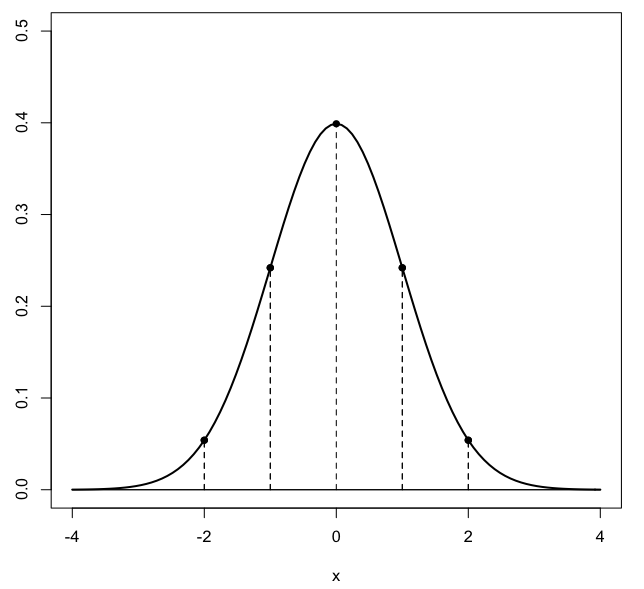
\includegraphics [scale=0.4] {gauss3.png} \end{center}

\begin{document}
\maketitle
\Large
\noindent

Ceva's Theorem says that if we start with a triangle and draw the line segments connecting each vertex with the midpoint of the opposite side, the three line segments cross at a single, unique point.  Furthermore, it is possible to show that for any of these line segments, the \emph{centroid} lies one-third of the length from the side, and two-thirds of the length from the vertex.

I'd like to show a proof of this using vectors, which makes everything particularly simple.  As a warmup, let's start by looking at the midpoint of the diagonals for a parallelogram including the triangle of interest.  We will prove that the two diagonals cross at their mid-points (at $P$).

 \begin{center} 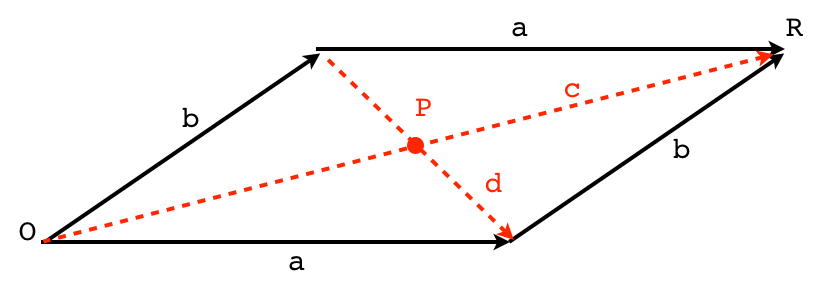
\includegraphics [scale=0.4] {ceva_vec1.png} \end{center}

by construction:

\[ \mathbf{c} = \mathbf{a} + \mathbf{b} \]
\[ \mathbf{b} + \mathbf{d} = \mathbf{a} \ \Rightarrow \  \mathbf{d} = \mathbf{a} - \mathbf{b}   \]

Let's define $P$ as the point we reach by going halfway along $\mathbf{c}$

\[  \mathbf{c} / 2 =  (\mathbf{a} + \mathbf{b})/2 \]

What we need to show is that if we do

\[ \mathbf{b} + \mathbf{d}/2 \]

we arrive at $P$.  Since $\mathbf{d} = \mathbf{a} - \mathbf{b}$

\[ \mathbf{b} + \mathbf{d}/2 = \mathbf{b} + (\mathbf{a} - \mathbf{b})/2 = (\mathbf{a} + \mathbf{b})/2 \ \ \ \  \blacksquare \]

Vectors make that pretty easy.

Now, here is the triangle.

 \begin{center} 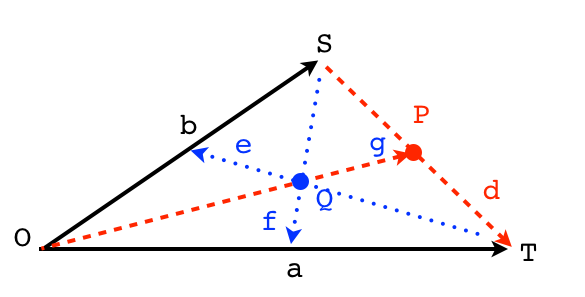
\includegraphics [scale=0.4] {ceva_vec2.png} \end{center}

By construction

\[ \mathbf{b} + \mathbf{f} =   \mathbf{a}/2 \ \Rightarrow \  \mathbf{f} =   \mathbf{a}/2 - \mathbf{b} \]
\[ \mathbf{a} + \mathbf{e} =  \mathbf{b}/2  \ \Rightarrow \  \mathbf{e} =   \mathbf{b}/2 - \mathbf{a} \]

Define $\mathbf{c}/2 = \mathbf{g}$

\[ \mathbf{b} + \mathbf{d}/2 =  \mathbf{g}\]

(For the last one, refer back to the first diagram).

It makes it a little easier when we know that $Q$ is two-thirds of the way along the line segment.  We have three paths to move to $Q$.

Starting from $O$:

\[ \frac{2}{3} \mathbf{g} = \frac{2}{3} \ \frac{1}{2} \mathbf{c} = (\mathbf{a} + \mathbf{b})/3 \]

from $S$:

\[ \mathbf{b} + \frac{2}{3} \mathbf{f} = \mathbf{b} +  \frac{2}{3}( \mathbf{a}/2 - \mathbf{b}) =  (\mathbf{a} + \mathbf{b})/3 \]

or from $T$:

\[ \mathbf{a} + \frac{2}{3} \ \mathbf{e} = \mathbf{a} + \frac{2}{3} \ (\mathbf{b}/2 - \mathbf{a}) =  (\mathbf{a} + \mathbf{b})/3 \]

How would we find the factor of $2/3$ if we didn't already know?  Call that unknown factor $r$

\[ r \ (\mathbf{a} + \mathbf{b})/2 + (1-r) \ \mathbf{e} = \mathbf{b} / 2 \]
\[ r \ (\mathbf{a} + \mathbf{b})/2 + (1-r) \ (\mathbf{b}/2 - \mathbf{a}) = \mathbf{b} / 2 \]
Expand:
\[ r (\mathbf{a}/2) + r (\mathbf{b}/2) + \mathbf{b}/2 - r (\mathbf{b}/2) -  \mathbf{a} + r  \mathbf{a} =  \mathbf{b}/2 \]
\[ r (\mathbf{a}/2)  + \mathbf{b}/2 -  \mathbf{a} + r  \mathbf{a} =  \mathbf{b}/2 \]\[ r (\mathbf{a}/2) -  \mathbf{a} + r  \mathbf{a} =  0 \]
\[ (3/2)r \mathbf{a} - \mathbf{a} = 0 \]
\[ (3/2)r  = 1 \]
\[ r = 2/3 \]

\end{document}  